\documentclass{llncs}
\pdfoutput=1

\usepackage{algorithm, algpseudocode}
\renewcommand{\algorithmiccomment}[1]{/*#1*/}
\usepackage{epsfig, endnotes, url, color, graphicx}
\usepackage{mathtools, amsmath, amsfonts}
\usepackage{diagbox, booktabs, colortbl}
\usepackage{breakurl, listings, framed}
\usepackage{multirow, caption, subcaption}
\usepackage[hidelinks]{hyperref}
\usepackage{xspace, slashbox, enumitem, bm}
\DeclareMathAlphabet{\mathcal}{OMS}{cmsy}{m}{n}

\pagestyle{plain}


\captionsetup[subfigure]{justification=raggedright}

\captionsetup{compatibility=false}
\def\UrlBreaks{\do\/\do-}
{\renewcommand{\arraystretch}{1.2}
\makeatletter
\newcommand{\@chapapp}{\relax}%
\makeatother

\usepackage[title]{appendix}

\newcommand{\tabitem}{~~\llap{\textbullet}~~}

\newcommand{\ignore}[1]{}
\newcommand\ghada[1]{\nbc{GA}{#1}{blue}}
\newcommand{\fake}[1]{{\color{magenta} [fake: #1]}}


\usepackage{ifthen}
\usepackage[normalem]{ulem} % for \sout
\usepackage{xcolor}
\let\lneq\undefined  % removes amssymb conflict with some packages
\usepackage{amssymb}
\newcommand{\ra}{$\rightarrow$}
\newboolean{showedits}
\setboolean{showedits}{true} % toggle to show or hide edits
\ifthenelse{\boolean{showedits}}
{
	\newcommand{\ugh}[1]{\textcolor{red}{\uwave{#1}}} % please rephrase
	\newcommand{\ins}[1]{\textcolor{blue}{\uline{#1}}} % please insert
	\newcommand{\del}[1]{\textcolor{red}{\sout{#1}}} % please delete
	\newcommand{\chg}[2]{\textcolor{red}{\sout{#1}}{\ra}\textcolor{blue}{\uline{#2}}} % please change
}{
	\newcommand{\ugh}[1]{#1} % please rephrase
	\newcommand{\ins}[1]{#1} % please insert
	\newcommand{\del}[1]{} % please delete
	\newcommand{\chg}[2]{#2}
}

\newboolean{showcomments}
%\setboolean{showcomments}{true}
\setboolean{showcomments}{true}
\newcommand{\id}[1]{$-$Id: scgPaper.tex 32478 2010-04-29 09:11:32Z oscar $-$}
\newcommand{\yellowbox}[1]{\fcolorbox{gray}{yellow}{\bfseries\sffamily\scriptsize#1}}
\newcommand{\triangles}[1]{{\sf\small$\blacktriangleright$\textit{#1}$\blacktriangleleft$}}
\ifthenelse{\boolean{showcomments}}
%{\newcommand{\nb}[2]{{\yellowbox{#1}\triangles{#2}}}
{\newcommand{\nbc}[3]{
 {\colorbox{#3}{\bfseries\sffamily\scriptsize\textcolor{white}{#1}}}
 {\textcolor{#3}{\sf\small$\blacktriangleright$\textit{#2}$\blacktriangleleft$}}}
 \newcommand{\version}{\emph{\scriptsize\id}}}
{\newcommand{\nbc}[3]{}
 \renewcommand{\ugh}[1]{#1} % please rephrase
 \renewcommand{\ins}[1]{#1} % please insert
 \renewcommand{\del}[1]{} % please delete
 \renewcommand{\chg}[2]{#2} % please change
 \newcommand{\version}{}}
\newcommand{\nb}[2]{\nbc{#1}{#2}{orange}}

\definecolor{jccolor}{rgb}{0.2,0.4,0.6}
\definecolor{clcolour}{rgb}{0.5,0.7,0.9}
\newcommand\cappos[1]{\nbc{JC}{#1}{jccolor}}
\usepackage{wasysym}




% Ghada: added to remove running headers
\pagestyle{plain}


\begin{document}
%
% paper title
\title{\Large \bf Rethinking Service Systems: \\
A Path Towards Secure and Equitable Resource Markets
}


\author{Ghada Almashaqbeh} 
%
\authorrunning{G. Almashaqbeh}
% First names are abbreviated in the running head.
% If there are more than two authors, 'et al.' is used.
%
\institute{NuCypher \\
\email{ghada@nucypher.com}}

\maketitle


\begin{abstract}
Escalating demand for digital services has motivated building non-traditional solutions to reduce costs and achieve a greater level of flexibility. Among these solutions, peer-assisted models are gaining more popularity in replacing infrastructure-based (possibly) centralized approaches. Cryptocurrencies have strengthened this trend by providing a fully distributed mechanism to compensate service provision, and their blockchains and consensus protocols offer a trustless and publicly verifiable way to govern the system. We present a generic framework for building distributed service markets by utilizing these new technologies. We also discuss the security and efficiency challenges, with a focus on how the economic considerations impact system design and threat mitigation, and conclude with some potential solutions.
\end{abstract}


\section{Introduction}
Usually, when obtaining digital services, we deal with traditional systems that are centrally managed. Most of the time, we resort to third party providers, e.g., commercial companies,  to obtain services like file storage, content distribution, computation outsourcing, and many others. Despite being effective and widely deployed, this centrally-managed paradigm introduces several trust, cost, and transparency issues. It requires establishing complex business relationships with these companies, where customers usually overprovision their needs in order to handle future peak demands~\cite{Kassa13,Nicolae14}. Also, it constrains the customers with the service specifications these companies can offer, like the geographic coverage and service speed, not to mention the limited visibility into the real status of the system regarding its performance and the available amount of resources.


These issues motivated the community to revisit old ideas of peer-to-peer (P2P) based models in which anyone is allowed to join the system and serve others. In order to encourage the collaborative work and compliance with the protocol, payments are provided in return, which creates a market for trading resources. This paradigm builds flexible systems, where customers can start or stop the service at any time. It also scales more easily with demand and extends the network coverage because peers from anywhere can join. Furthermore, this paradigm builds transparent and equitable ecosystems in which participants can negotiate service terms and price directly instead of having a few entities monopolizing the market.


\begin{table}[t!]
\caption{Examples of centrally-managed digital services and their counterparts of P2P-based ones.} 
\label{service-examples}
%\vspace{-10 pt}
\centering 
\begin{tabular}{| p{0.32\columnwidth}  | p{0.32\columnwidth} | p{0.32\columnwidth} |}\hline\hline

{\bf Service Type} & {\bf Traditional Solution} & {\bf P2P-based Solution}  \\[0.5ex] \hline \hline
 
Payments & Banks & Bitcoin  \\[0.5ex] \hline

File storage & Dropbox~\cite{dropbox} &  Filecoin~\cite{filecoin}  \\ [0.5ex]  \hline   

Content distribution & Akamai~\cite{akamai} & CacheCash~\cite{almashaqbeh2019cachecash}  \\ [0.5ex]  \hline
    
Key management system & Azure Key Vault~\cite{azure} & NuCypher~\cite{nucypher}  \\ [0.5ex]  \hline    

\end{tabular}
\end{table} 



Although monetary-incentivized P2P-based systems are an old idea, especially for content sharing, most of existing solutions introduce some form of centralization or trust. They either rely on centralized payment services, place trust in specific parties to handle these payments and solve disputes, or even rely on some centralized entities to manage participants and defend against some security threats~\cite{Kassa13,Nair08,Zhang09}. Such design choices bring us back to the central management model and the trust issues of traditional solutions.


The evolution of cryptocurrencies and blockchain technology~\cite{bitcoin,ethereum} has provided templates for reshaping large-scale distributed systems and services. Cryptocurrencies implement a decentralized virtual currency exchange medium that permits participants to be rewarded without any pre-authentication or identification requirements. And their underlying blockchains and consensus protocols support public verifiability, auditing, and decentralized governance without needing to place trust in any entity. These features can be exploited in P2P-based schemes to manage and pay for the correct service without driving the system toward centralization (see Table~\ref{service-examples} for examples of traditional service solutions and their P2P counterparts).


However, the open access environment of P2P networks (i.e., allowing anyone to join and dealing with untrusted participants) introduces several security and performance challenges that need to be addressed before having any practical deployment. In addition, having monetary incentives motivates attackers to attack the system in novel ways to maximize their financial profits. Thus, traditional practices of secure systems design need to be modified and expanded to account for such factors.


To address these issues, in this talk we present a generic framework for designing secure, scalable, and equitable resource markets to provide services in a fully distributed way. This framework accounts for the economic aspects of this service paradigm covering both market viability (compared with traditional ones) and the impact of monetary incentives on system security (in terms of identifying financially-motivated threats and building economic or game-theoretic mitigation techniques). We conclude with zooming on one of the important security facets of monetary-incentivized decentralized services, namely, addressing accounting attacks, i.e., how to prove that service has been delivered, or alternatively payments are well deserved. We elaborate on our experience in designing distributed access control services at NuCypher~\cite{nucypher} and the solutions we developed to thwart these attacks. We also show how the financial motivations of attackers vary based on the operation stage of the network (early launch vs. long term operation) and how threat mitigation techniques vary accordingly.


\section{Distributed Resource Markets Design}
One of the effective ideas for building fully decentralized and equitable services is to build distributed markets to trade resources. That is, implement a protocol that allows anyone to join to serve others and collect payments in return. Such an approach needs to solve several challenges introduced by the open access and decentralized work environment. In other words, dealing with untrusted, possibly financially motivated participants requires deploying additional measures that may impact efficiency, usability, and compatibility with existing infrastructures. Consequently, there is a need for carefully-tailored threat mitigation techniques and efficiency optimization mechanisms in order to promote the adoption of these systems.


\begin{figure}[ht!]
\centerline{
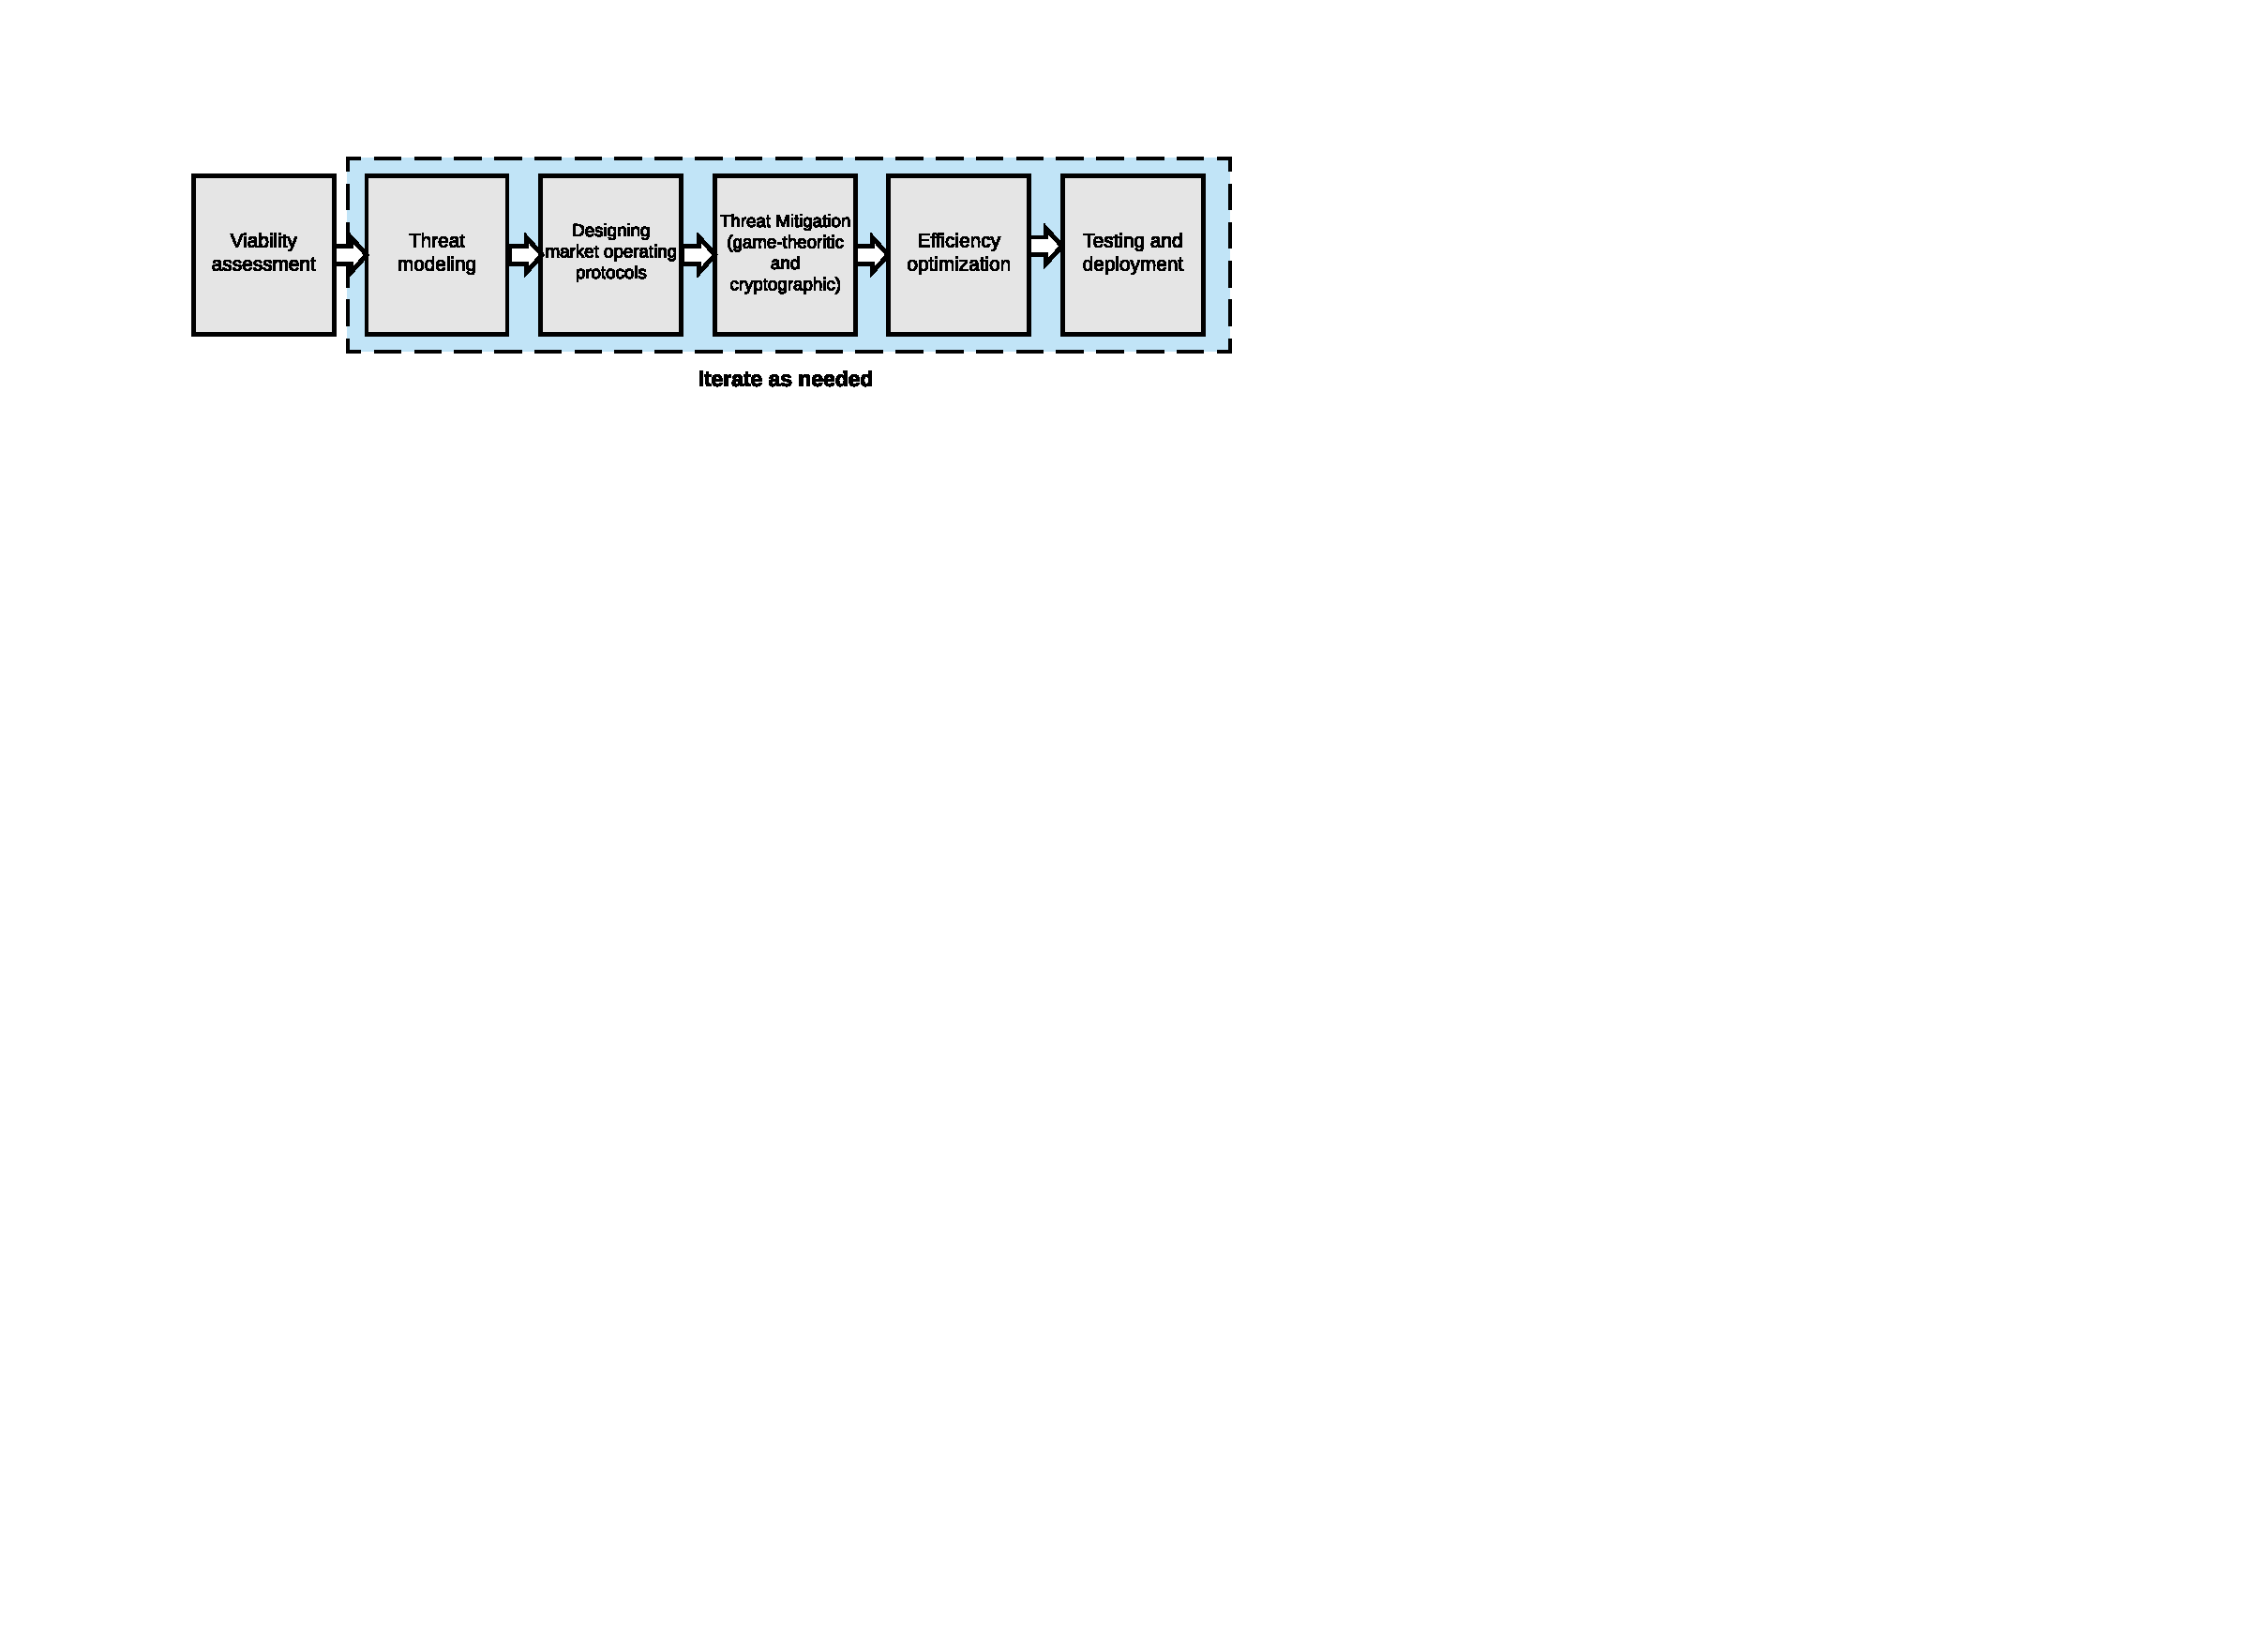
\includegraphics[height= 1.2in, width = 1.0\columnwidth]{figures/design-steps.pdf}}
\caption{Design process of distributed resource markets.} \label{design-steps}
\vspace{-12pt}
\end{figure}


In this section, we discuss the main steps and challenging issues that need to be considered when designing a distributed service system. These steps are captured at a high level in Figure~\ref{design-steps}, which we discuss in greater details in the following paragraphs. \\


\noindent{\bf Viability Assessment.} Before looking into building a distributed resource market, one has to assess its viability. This includes studying the demand side (who is interested in the service) and the supply side (who can provide it) to answer several questions; Are there tangible advantages to encourage replacing traditional solutions with fully distributed ones? Can the system match the reliability and performance offered by these traditional solutions? and does providing the service require large amounts of resources that exceed the capabilities of average end-users? Such a viability study is an important step to assess the potential for practical adoption before investing time and effort into building the system. \\


\noindent{\bf Threat Modeling.} Despite the many advantages they offer — decentralization, transparency, and lowered service costs — there is still a big gap between the promise of P2P-based systems and their performance in practice. Adding monetary incentives, by using another P2P-based payment service, i.e., cryptocurrencies, widens this gap. This is due to the perception that these systems are not secure, where the recent large number of security breaches give credence to these doubts~\cite{benebit-scam,binance-hack,bitcoin-cash-hack,bitcoingold-double-spending,exchange-hack-b,bitfloor-hack,korea-exchange-hack,eth-hack,ico-hack-b,exchange-hack,enigma-hack,mine-hack}.


The best practice for designing a secure system requires a threat modeling step to investigate potential security risks. Such a model can guide designers in deploying the proper countermeasures, and evaluating the security level of a system. For resource markets, building a threat model requires a framework that can handle large-scale distributed systems, explicitly account for the financial motivations of the attackers, and help in spotting any potential collusion or sybil attack.


This observation encouraged the community to visit old threat modeling frameworks and adapt them to address these issues. For example, the ABC framework~\cite{Almashaqbeh19} was designed to achieve these goals by accounting for both the underlying cryptocurrency medium and the service provided on top of it. ABC enables building comprehensive threat models by holistically analyzing the threat space while managing its complexity, and distilling the impactful cases that need to be neutralized to secure the system. It also allows classifying threats based on their mitigation techniques, i.e., threats that can be addressed cryptographically or algorithmically, and these that require game theoretic means, thus providing insights about the proper measures to deploy.


It should be noted that the threat modeling steps need to be revisited each time the system design is altered. Furthermore, it should be performed as the last step before shipping the system to argue formally about its security.  \\


\noindent{\bf Unique Aspects of Operating a Distributed Market.} The open access work environment helps to create flexible services and transparent ecosystems. However, this comes at a cost. Dealing with untrusted parties means that fair exchange is impossible~\cite{Even80,Pagnia99}, which raises the question of when to pay service-providers - before or after providing the service? If paid first, a malicious service-provider may not serve the customer, and if served first, a malicious customer may not pay afterwards.


Furthermore, accounting attacks, in which participants collude with each other pretending that the service has been delivered, could be a hammer that may destroy the market. This is a particular problem in systems that require sponsoring service requests. For example, in content distribution, a publisher (e.g., Netflix) can hire caches to distribute content to its clients, and hence, it pays for the service. In this case, caches (or service-providers in general) and clients may collude so that clients pretend to be served, allowing service-providers to collect payments from the sponsor for free.


The above security issues (an many others depending on the service type) require a careful design of a decentralized service-payment exchange protocol that can reduce the risks of dealing with untrusted, possibly colluding parties. Such a protocol represents the backbone of the resource market; if it fails the whole market fails. Service-providers will not be willing to participate if they are not being paid, and same for customers, they will not be willing to use the system if they pay for a service that they do not receive. Operating the market also requires devising mechanisms for service pricing, term negotiation for service-provider recruiting, and matching protocols to match these service-providers with interested customers. \\


\noindent{\bf Financial and Cryptographic Security Measures.} Usually, security threats are mitigated by using cryptographic means (e.g., encryption and digital signatures), or algorithmic approaches (e.g., ordering the actions in a way that enforces secure behavior). Monetary-incentivized systems introduce new types of attacks that cannot be addressed using conventional approaches. In particular, having financially-motivated attackers introduces new threat vectors that need to be mitigated by using financial means. These fall into three categories: first, detect-and-punish mechanisms, where any participant is required to lock collateral that is forfeited if he/she is caught cheating. Second, designing algorithms that, if performed maliciously, require larger amounts of resources than when performed honestly. And third, designing service pricing and payments mechanisms that make it more profitable on the long run to act honestly in every service request than cheating or ignoring the request (even if cheating or ignoring are not detectable). Such techniques make cheating unprofitable so that the majority of rational parties will choose to follow the protocol.


For example, to reduce the risks of the impossibility of fair exchange, micropayments can be employed. That is, instead of paying a large chunk of money for the full service, the payment is divided into small values, each of which is exchanged for a small service amount. For instance, one can pay for retrieving a file in small data chunks instead of paying for the full retrieval all at once. Hence, a service-provider loses a small payment if a client does not pay after receiving a chunk. Similarly, a client loses a small payment if it pays in advance and the service-provider does not send a data chunk in return.


On the other hand, to thwart accounting attacks, system designers need to incorporate suitable techniques to prove or confirm resource expenditure, and consequently, confirm that payments are well deserved. In online content delivery, for example, the CAPnet puzzle~\cite{Almashaqbeh19b} can be used to ensure that caches have delivered the requested content. The design of this puzzle follows the second category mentioned above, where solving the puzzle without doing the work is more expensive (resources-wise) than solving it after retrieving the content. In file storage, proof-of-replication~\cite{Fisch19} can be used to prove that a service-provider is still storing the clients’ files with the agreed-upon number of replicas. Here, a detect-and-punish mechanism is used, where failing in providing a correct proof leads to slashing part of the deposit a service-provider pledged when joining the system~\cite{filecoin}. Thus, the type of the provided service directly influences the mechanisms for delivery confirmation, compensation and punishment that need to be deployed. \\


\noindent{\bf Optimize for Efficiency.} Although designing a secure system is the ultimate goal, efficiency is an important driving factor of practical adoption and deployment. System designers need to exploit any opportunity that allows for optimizing performance. This also involves choosing the right trade-off between security and efficiency in the sense of risk management. That is, threats that have high impact need to be prioritized over low impact ones. Moreover, looking into alternative cryptographic primitives that are lightweight, or optimize their implementation, while maintaining the required security guarantees is another effective avenue to utilize.


Furthermore, reducing interaction between participants is beneficial. It speeds up the service and promotes the system’s scalability. This can take the form of batching requests/replies between customers and service-providers to reduce costs and optimize resource allocation, in addition to batch or aggregate record verification on the blockchain.


Another important aspect is related to handling micropayments. Micropayments create a scalability problem as they produce a huge number of transactions that overwhelm the system and require large processing fees. Here, probabilistic schemes are useful in aggregating the small transactions into few larger ones before processing~\cite{Wheeler96,Rivest97}. In particular, payments take the form of lottery tickets, and only winning tickets are processed in the system with values that compensate properly for the tickets exchanged so far. Several fully-distributed micropayment schemes exist in the literature~\cite{Pass15,Chiesa17,Almashaqbeh20} that provide trade-offs between efficiency, anonymity, and security guarantees. \\


\noindent{\bf Testing and Deployment.} To examine the viability of the system, conventional practices of prototyping, benchmarking, and controlled deployment can be used to evaluate both efficiency and resistance to attacks. These provide a starting point to attract early adopters and test the system at a large scale. This stage may inspire designers to revisit specific parts of the system for further optimization based on the results of the conducted experiments, or feedback from the community based on a testnet deployment for example. Testing and improving also continue beyond the testing stage, i.e., after public launch, but deploying protocol modifications could be harder especially if they result in hard forks or community division.


\section{Impact of Financial Incentives on Service Delivery}
\vspace{-4pt}
In this section, we elaborate on one of the important issues in distributed resource markets, namely, service delivery. We examine how financial incentives affect which technique to deploy in order to enforce the honest behavior of the service-providers. In particular, we report on some work we have done in the NuCypher network under the umbrella of confirming service-providers' activity. We show how early stages of network launch differ from later periods when the network is stable, particularly in terms of reward computation, which in turn impact the financial motivations of attackers. Such an issue is a great example of how cryptocurrency-based services introduce new economic aspects that may evolve over time, which need to be reflected on the system design. \\


\noindent{\bf An overview of the NuCypher network.} The NuCypher network~\cite{nucypher,egorov2017nucypher} is a decentralized key management
system, encryption, and access control service. It uses proxy re-encryption, namely, the
Umbral scheme~\cite{umbral2018}, to delegate access to encrypted
documents through a public network. This network is composed of a set of semi-trusted
re-encryption service-providers, or Ursulas, that implement access control policies created by data
owners, or Alices. Alice supplies each Ursula with re-encryption keys allowing Ursula to transform
ciphertexts encrypted under Alice's public key into ciphertexts encrypted under the delegatee's, or Bob's,
public key. This enables the latter to decrypt the ciphertext without revealing anything about the
decryption keys or the raw data to the intermediate service-providers.


Joining the NuCypher network is governed by consensus rules defining the service setup
and the monetary incentives paid to provide the service. In order to join the 
system, Ursula needs to stake an amount of NU tokens (the native token of the network) for a specific period
which will be released when the pre-specified staking period is over. Alice chooses an
Ursula to hold an access control policy with a probability proportional to the stake this Ursula 
pledged in the system. Therefore, the stake value influences the service load an Ursula
may receive. This stake is also used to punish Ursula financially, by forfeiting part
of it, if she cheats and this cheating is detected. 


Alice joins the network by creating a policy to be implemented by a 
set of Ursulas. This policy specifies the re-encryption key fragments each Ursula will
need to answer requests coming from Bob(s), as well as the duration of the policy, which 
is basically the timeframe during which Bob is authorized to access Alice's data.  Furthermore,
Alice will lock an amount of Ether into the policy contract to be used to pay Ursulas for the re-encryption 
service. As noted, Alice is not exposed to the NU token. All that she needs is an Ethereum
wallet, awareness of the NuCypher network architecture to select Ursulas, and knowledge of the
NuCypher rules of preparing access control policies.


Bob, on the other hand, does not deal with currency in the system at all. He interacts with the storage 
network to retrieve the encrypted data, and with Ursulas in the NuCypher network to request the
re-encryption service. \\


\noindent{\bf Monetary incentives in the NuCypher network.} Ursulas are rewarded for the re-encryption service by using two sources; the first is the service fees collected from the policy owner Alice, while the second is a subsidy in the form of newly minted NU tokens distribted on a schedule enforced by the NuCypher protocol. The latter will be provided during the early stage of the network operation to encourage service-provider participation and sustain their operations in lieu of a mature fee market.

Currently, the subsidy size in each round or period are computed for each Ursula based on the size of her stake and duration of commitment to the network, and provided that she confirms to be online during this round. Confirming the status of being online is done by calling a simple function in one of the NuCypher contracts, which is like a signal that the calling Ursula is online. Similarly, for fees, Ursula collects part of the Ether locked by Alice during the policy's duration in proportion to the number of periods up to that point in which Ursula has confirmed her online status.


Although subsidy computation and collection based on activity monitoring is reasonable for the first iteration of the network, we acknowledge that it suffers from two main problems:
\begin{itemize}
\setlength{\itemsep}{0pt}
\item The revenue computation (both fees and subsidies) is agnostic to the number of requests Ursula serves. Thus, an active Ursula who may serve a huge number of re-encryption requests, and one who does not receive any requests (or more importantly, a malicious/lazy Ursula that does not answer Bob's requests), will both collect the same amount of revenue if they hold identical policies.

\item Confirming being online is flawed in the sense that this function does not require any input or proofs from Ursula on providing the service. Ursula can stay offline the majority of the time and not respond to Bobs' requests, then come online merely to call the confirm activity function. This allows Ursula to collect both subsidies and fees without doing all (or even most) of the necessary work. Even worse, Ursula will be able to get her stake back once it unlocks.
\end{itemize}


Therefore, we need to devise a secure, non-gameable technique that confirms Ursula's minute-to-minute availability and service activity. Then we need to adapt the subsidy and fee computation accordingly to factor in the amount of delivered service, and potentially punish Ursulas if it is insufficient. These are introduced in the rest of this section. \\


\noindent{\bf Problem definition based on network operation stage.} The confirm activity problem is defined differently based on the stage of the network operation. In the first 5 to 8 years after launch, when subsidy rewards are
still distributed, we are concerned with the availability of Ursulas and their willingness to
serve all requests coming from Bob. In other words, regardless of the number of requests served, the revenue total (both subsidies and fees) will be computed based on the length of time in which Ursula
is online and well-behaved. In later stages, when subsidies disappear
and the only revenue comes from fees, confirm activity will be tied to providing the re-encryption
service, in the sense that the payment will be partially computed based on the amount of
service provided. This requires Ursula to confirm its activity by proving that she served 
a given number of distinct re-encryption requests during a given period. To make the distinction 
clear, we refer to the first as \emph{confirm availability}, and for the second as \emph{confirm 
service activity}. \\


\noindent{\bf Confirm availability and service activity solutions.} In~\cite{confirm-activity-draft}, we introduce several solutions for both forms of the above problem. These solutions differ with respect to trust, efficiency, interactivity, and resource requirements, in addition to their security guarantees, which we present briefly in what follows. Before that, we review the adopted threat model.


\paragraph{Threat model.} We do not place trust in any party and we assume that all participants are rational and self-interested. Thus, they may follow the protocol or deviate from it, either acting on their own or in collusion with each other, based solely on what maximizes their utility gain. 


However, we argue that collusion between Bob and Ursula to perform accounting attacks (i.e., Bob pretends that service has been delivered allowing Ursula to collect payments for free) is not economically advantageous, and hence, not an issue in our system. The reason is that the amount of work an Ursula does when replying to a re-encryption request is minimal. This means that colluding with Bob to fake re-encryptions will save minimal resources and has no clear economic gain (such as extra subsidies), which makes this collusion case unappealing to rational Ursulas. This case is a great example of how traditional threat modeling and risk management practices differ from those economic-oriented ones in ruling out financially-inefficient threats.


Moreover, we assume that when sampling a subset of Ursulas in the network, at least one of them is honest. This assumption can be achieved by having a global assumption regarding the lower bound of the number of 
honest Ursulas with respect to the total number of Ursulas in the system.\footnote{Or it can be achieved by deploying a special entity like an external verifier, that changes on a periodic basis, or one by the NuCypher company, that is trusted to faithfully participate as a member of each sampled set. This verifier does not provide any other services in the system.}


\paragraph{Confirm availability solution.} Here we use a detect-and-punish approach embedded within an optimistic service monitoring process. This means that it is only invoked when Bob complains that an Ursula is unresponsive. In detail, for each round\footnote{A round is the time needed to mine a block or several blocks on the underlying blockchain.} a set of Ursulas is selected at random to act as gateways (or service watchers).\footnote{One approach to do that in a distributed way is to feed a random beacon (like block hashes in the random oracle model) to an iterative hashing process. Then map each hash to an Ursula index as found in the list of working Ursulas recorded on the blockchain within the StakeEscrow smart contract of NuCypher. This process is repeated until a set of distinct Ursulas is selected. Note that anyone can perform this process and verify its outcome.} Bob proceeds as usual by contacting the list of working Ursulas received from Alice for the re-encryption service. If a working Ursula does not reply, Bob complains to a gateway Ursula and hands her the request. This gateway mediates the service process in order to check if Bob's claim is valid. In other words, she challenges the working Ursula by forwarding the request again and waiting for an answer (which must arrive within a specified, universal time window). If one is received, the gateway forwards it to Bob and closes the complaint.


On the other hand, meaning no response is received, the gateway notifies the rest of gateways selected for that round to repeat the same process. If no response is received by any of them, the quorum signs a proof-of-unavailability (e.g., by using collective signing~\cite{syta2016keeping}) against the working Ursula stating that she is unavailable and submit this proof to the NuCypher staking contract. At that time, a part of the working Ursula stake is slashed (with a minimum value derived based on the additional utility gain an Ursula collects by faking to be online) as a punishment. This punishment makes cheating unprofitable, and hence, unappealing to rational working Ursulas. A detailed technical version of this solution is available in~\cite{confirm-activity-draft}.


As long as Ursula is behaving well and no valid complaints from Bob, this Ursula will collect both subsidies and service fees in proportion to her availability period and the number of policies she holds. In other words, revenue computation follows the same current approach outlined earlier since our concern is to encourage adoption especially when service demand is low at the beginning.


\paragraph{Confirm service activity solutions.} Here we have three solutions that differ in their security assumptions and efficiency. We refer to them as zero knowledge proof-based (ZKP-based), committee-attestation, and commit/challenge/open-based. Again, we provide a high level description in what follows while a more complete version can be found in~\cite{confirm-activity-draft}. 


As for the \emph{ZKP-based} solution, in the NuCypher network each Ursula produces a zero knowledge proof attesting to the correctness of the re-encryption she performed to be checked by Bob~\cite{umbral2018}. We can combine the proofs of all served requests within a round into one attesting to the following statement: "An Ursula has served $\omega$ distinct requests correctly" for some positive integer $\omega$ representing the number of served requests. This accumulation can be done by using generic techniques like proof carrying data (PCD)~\cite{chiesa2010proof} or incrementally verifiable computation (IVC)~\cite{valiant08}.


An alternative, possibly more efficient approach is to view the statement "An Ursula has served $\omega$ distinct requests correctly" as an instance of the arithmetic circuit satisfiability problem and utilize bulletproofs\footnote{Bulletproofs are a highly efficient ZKP system that does not require any trusted setup.} to prove its correctness in zero knowledge~\cite{bunz18}. That is, build a circuit that takes the set of correctness proofs of the served requests as well as their number $\omega$ as inputs, and then output 0 if number of correct distinct proofs equals to $\omega$. Then, invoke a circuit parser to convert the circuit into the bulletproof format, which allow the prover, Ursula in this case, to produce a single proof. Then, Ursula submits the proof to the service policy contract. Once the proof is verified, the contract disperses the service fee (in proportion to $\omega$) from Alice's escrow to Ursula's account.


As for the \emph{committee-attestation} approach, it also relies on electing a committee of Ursulas (and possibly outsider verifiers as mentioned previously) to attest for the work load an Ursula served. That is, a working Ursula sends all Bob requests she served along with the correctness proofs to this committee. After verifying all the proofs, the committee collectively signs a statement as above which is submitted to the policy contract so Ursula can claim her payment.


Lastly, we have a \emph{commit/challenge/open} approach, which is inspired from the Merkle tree-based ZKP system proposed in~\cite{dottling19}. Ursula constructs a Merkle hash tree of all served requests and their correctness proofs in a round. Then, it uses the root as a random beacon to be fed into an iterative hash process to select $n$ leaf nodes at random to open them (i.e., these are the challenges). Ursula signs the Merkle tree root, provides the challenge leaf nodes along with their membership paths to either a sidechain (which is maintained by round-selected committee) or to the policy contract to verify. As noted, the security provided here is statistical in the sense that we need to bound the probability by which an Ursula can cheat, like for example she may replicate requests in the tree and add fabricated ones to increase $\omega$. 


\paragraph{Discussion.} Which solution to adopt will be based on benchmark testing and the development vision of the NuCypher network. The ZKP-based solution (the one utilizing bulletproofs) provides several advantages including non-interactivity (as opposed to the committee-attestation one that needs interaction with the committee). It also supports computational soundness as opposed to the statistical one of the commit/challenge/open solution. Nonetheless, it could be the case that the other solutions are more efficient especially if we incorporate committee attestation or sidechains to support other functionalities in the network. 


Another issue is regarding the payment computation. During early stages when the network launches, we anticipate a limited adoption and service demand. Thus, we reward Ursulas for just being online to encourage adoption. While in later stages, payments will be dispensed partially in proportion to the actual amount of service requests an Ursula answers. This is due to the fact that later on the subsidies will effectively disappear, i.e., the majority of tokens in the network will be minted, and the service fees are the only source of income. To incentivize Ursula to provide a correct and timely service, these fees should be computed based on the actual amount of service. This shows how changes in incentive alignment lead to different views on how to distribute these incentives and ensure the security of the system.


\section{Conclusion}
While centrally-managed systems provide reliable services, they introduce trust, cost, and transparency issues. This motivated developing non-traditional peer-assisted models to create distributed resource markets that are open to anyone to join and serve others while collecting payments in return. However, such a paradigm comes with security and performance challenges that need to be addressed before having any practical deployment. Our work puts forward a generic framework for designing efficient and secure resource markets. It also examines in a greater depth how financial incentives affect security measures deployment and system design choices.


{\footnotesize \bibliographystyle{acm}\vspace{-6pt}

\bibliography{marketBib}}

\normalsize

% that's all folks
\end{document}


